% TikZ code representing 2-colorability examples:
% Left: a 2-colorable graph with a valid 2-coloring.
% Right: a non 2-colorable graph with an odd cycle highlighted in red.

% ==================== PARAMETERS ====================
% Colors for nodes and highlights
\providecommand{\colorNodeA}{blue!60!white}        % Color A for valid 2-coloring
\providecommand{\colorNodeB}{orange!75!white}      % Color B for valid 2-coloring
\providecommand{\colorNeutral}{white}              % Neutral fill for uncolored nodes
\providecommand{\colorHighlight}{red!80!black}     % Color for highlighted odd cycle

% Dimensions and Line Thicknesses
\providecommand{\nodesize}{15pt}                   % Diameter of graph nodes
\providecommand{\edgethickness}{0.9pt}             % Thickness of standard edges
\providecommand{\highlightthickness}{2.2pt}        % Thickness of highlighted odd cycle edges
\providecommand{\nodeborderthickness}{0.9pt}       % Thickness of node borders

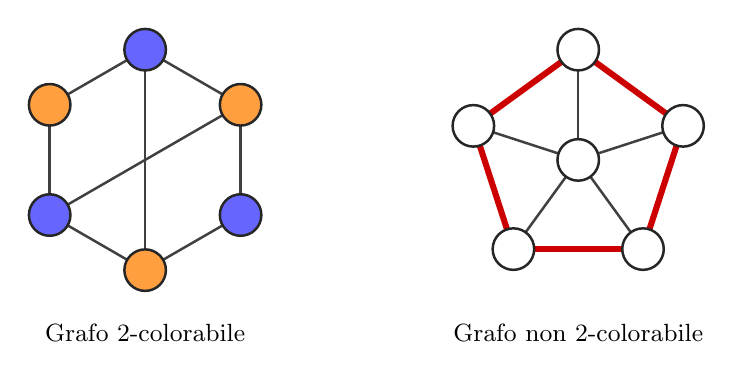
\begin{tikzpicture}[
    scale=1.0,
    % Node styles
    node_base/.style={
        circle,
        draw=black!85,
        line width=\nodeborderthickness,
        minimum size=\nodesize,
        inner sep=0pt
    },
    node_neutral/.style={node_base, fill=\colorNeutral},
    node_colorA/.style={node_base, fill=\colorNodeA},
    node_colorB/.style={node_base, fill=\colorNodeB},
    % Edge styles
    normal_edge/.style={
        line width=\edgethickness,
        draw=black!75
    },
    highlight_edge/.style={
        line width=\highlightthickness,
        draw=\colorHighlight
    },
    sublabel/.style={
        font=\small,
        align=center
    }
]

    % ==================== LEFT GRAPH: 2-colorable (Valid 2-coloring) ====================
    % Hexagon vertices centered around (0, 0)
    \coordinate (u1) at ({1.4*cos(90)},  {1.4*sin(90)});
    \coordinate (u2) at ({1.4*cos(30)},  {1.4*sin(30)});
    \coordinate (u3) at ({1.4*cos(330)}, {1.4*sin(330)});
    \coordinate (u4) at ({1.4*cos(270)}, {1.4*sin(270)});
    \coordinate (u5) at ({1.4*cos(210)}, {1.4*sin(210)});
    \coordinate (u6) at ({1.4*cos(150)}, {1.4*sin(150)});

    % Edges of 2-colorable graph (drawn first)
    \draw[normal_edge] (u1) -- (u2);
    \draw[normal_edge] (u2) -- (u3);
    \draw[normal_edge] (u3) -- (u4);
    \draw[normal_edge] (u4) -- (u5);
    \draw[normal_edge] (u5) -- (u6);
    \draw[normal_edge] (u6) -- (u1);
    % Internal chords between opposite vertices (distance 3, valid bipartite connections)
    \draw[normal_edge] (u1) -- (u4);
    \draw[normal_edge] (u2) -- (u5);

    % Draw 2-colored nodes over edges
    % Color A (u1, u3, u5)
    \node[node_colorA] at (u1) {};
    \node[node_colorA] at (u3) {};
    \node[node_colorA] at (u5) {};

    % Color B (u2, u4, u6)
    \node[node_colorB] at (u2) {};
    \node[node_colorB] at (u4) {};
    \node[node_colorB] at (u6) {};

    % Sublabel for left graph
    \node[sublabel] at (0, -2.2) {Grafo $2$-colorabile};


    % ==================== RIGHT GRAPH: Non 2-colorable (Wheel W_5) ====================
    % Wheel graph W_5 centered around (5.5, 0)
    % 5 outer vertices in a regular pentagon + 1 center vertex
    \coordinate (v0) at (5.5, 0);
    \coordinate (v1) at ({5.5 + 1.4*cos(90)},  {1.4*sin(90)});
    \coordinate (v2) at ({5.5 + 1.4*cos(162)}, {1.4*sin(162)});
    \coordinate (v3) at ({5.5 + 1.4*cos(234)}, {1.4*sin(234)});
    \coordinate (v4) at ({5.5 + 1.4*cos(306)}, {1.4*sin(306)});
    \coordinate (v5) at ({5.5 + 1.4*cos(18)},  {1.4*sin(18)});

    % Radial spokes to center (drawn first)
    \draw[normal_edge] (v0) -- (v1);
    \draw[normal_edge] (v0) -- (v2);
    \draw[normal_edge] (v0) -- (v3);
    \draw[normal_edge] (v0) -- (v4);
    \draw[normal_edge] (v0) -- (v5);

    % Highlighted odd cycle C_5 outer edges (bolder and red)
    \draw[highlight_edge] (v1) -- (v2);
    \draw[highlight_edge] (v2) -- (v3);
    \draw[highlight_edge] (v3) -- (v4);
    \draw[highlight_edge] (v4) -- (v5);
    \draw[highlight_edge] (v5) -- (v1);

    % Draw neutral nodes over edges
    \node[node_neutral] at (v0) {};
    \node[node_neutral] at (v1) {};
    \node[node_neutral] at (v2) {};
    \node[node_neutral] at (v3) {};
    \node[node_neutral] at (v4) {};
    \node[node_neutral] at (v5) {};

    % Sublabel for right graph
    \node[sublabel] at (5.5, -2.2) {Grafo non $2$-colorabile};

\end{tikzpicture}
